\documentclass[conference]{IEEEtran}
% \IEEEoverridecommandlockouts
% The preceding line is only needed to identify funding in the first footnote. If that is unneeded, please comment it out.
\usepackage{cite}
\usepackage{amsmath,amssymb,amsfonts}
\usepackage{algorithmic}
\usepackage{graphicx}
\graphicspath{{images/}}
\usepackage{float}
\usepackage{textcomp}
\usepackage{xcolor}
\usepackage{hyperref}
\def\BibTeX{{\rm B\kern-.05em{\sc i\kern-.025em b}\kern-.08em
    T\kern-.1667em\lower.7ex\hbox{E}\kern-.125emX}}
\begin{document}

\title{Combating Cognitive Bias in Financial Decision-Making with Regime Detection \\
% {\footnotesize CS 6795: Cognitive Science - Summer 2024}
%{\large CS 6795: Cognitive Science - Summer 2024}
}

\author{\IEEEauthorblockN{John Houck}
jhouck8@gatech.edu \\
}

\maketitle


% -------------------------- body ------------------

\begin{abstract}
In financial markets the common wisdom is to hold your investments for the long term. Historically, this approach has great upside, but it requires a lot of discipline on the part of the investor. 

In the information rich world we live in, investors can be swayed from their long-term financial plan, and unfortunately most investors tend to buy when the market is near its high point and sell when it is at a low point. Fear takes over and the average investor loses a lot of money selling and buying at the wrong time. In this paper, I explore a computational tool that I've written to help the average investor become more aware of market regime shifts with the goal of helping investors avoid selling when the market is near the bottom or buying when the market is the near the top. 

Reggie, as my application is called, is designed to help investors profit by buying low and selling high. 
\end{abstract}


\section{Introduction}

Reggie is a computational tool designed to help the average investor avoid the many pitfalls and cognitive biases inherent to investing. The name Reggie is a short form of the financial term regime change. This playful name gives a bit of character to a rather technical sounding financial term. In Financial markets, regime changes happen when the market suddenly shifts in a profound way. The shift in the market could be a change from a bull to a bear market. Another example is a substantial change in inflation that may precipitate a regime change. At the most basic level, regime change happens when there are structural changes in a time series. Often, these structural changes in the time series of stock prices indicate a dramatic shift in the market.

Fear often derails the average investor. During a stock market crash the average investor sells because they fear the market will drop further and further and on the other hand, fear of missing out often leads the average investor to buy near the top of a stock market run. Reggie is designed to remind investors that buying high and selling low is an unprofitable strategy. 

There is no way to predict the direction of the stock market, but by having a simple tool that can determine if there is a regime change occurring the hope is that investors can be more aware of the market and use this knowledge to buy low and sell high, or to at least stay the course and keep their investments in place. It's important to have a way to signal regime changes so that investors can have the proper perspective when there are large shifts in the market. The goal of Reggie is to make this kind of regime change forecasting available in the form of a simple application that an average retail investor could have on their phone.


\section{Computational Tool Design}

Reggie uses hidden Markov models to detect regime changes from historic price data. Hedge funds use sophisticated regime change machine learning algorithms to time their trades. The London Stock Exchange Group recently released a paper that goes in-depth exploring the various methods that can be used for regime detection and the benefits of each. \cite{b3} They conclude in the article that Hidden Markov Models are the most effective method for regime detection and Reggie uses some of this code for its regime detection. This method of regime detection is not something most retail investors have access to.

If an investor understands the cognitive science behind the fear-based trade of buying high and selling low, they can take a more contrarian approach when there are regime changes in the market. Ultimately, buying when there is ``blood in the streets'' as outlined by Daniel Myers has been shown to create tremendous upside. \cite{b2} Reggie also has a database of inspirational quotes from famous investors and a new one is shown every time the application is started, see Figure \ref{fig:fig1}. This appeals to the more emotional side of investing as showing the user only the data may not be enough to shift their behavior.

Another indicator used in the design of Reggie is known as the ``VIX''. It is also known as the fear index. Here is how Investopedia defines it: ``The CBOE Volatility Index, or VIX, is a real-time market index representing the market's expectations for volatility over the coming 30 days. Investors use the VIX to measure the level of risk, fear, or stress in the market when making investment decisions.'' \cite{b8}

In addition to the VIX and regime detection, technical analysis can be helpful in guiding investors. The problem with many brokerage applications is that they allow the user to add way too many different technical indicators to a chart. It's overwhelming and most seasoned traders and investors tend to use just a handful of technical indicators that they know well. The technical indicators that Reggie uses are 50/200 simple moving average, Bollinger Bands, Stochastic Oscillator, and Relative Strength Index. 

The 50-day and 200-day simple moving averages smooth out the historic price data and allow the user to see the trend from the noise of daily fluctuations. Investopedia states, ``The 200-day simple moving average is considered such a critically important trend indicator that the event of the 50-day SMA crossing to the downside of the 200-day SMA is referred to as a `death cross,' signaling an upcoming bear market in a stock, index, or other investment.'' In a similar fashion when the market is poised to rise, ``In like fashion, the 50-day SMA crossing over to the upside of the 200-day SMA is sometimes called a `golden cross,' referring to the fact that a stock is considered golden, or nearly sure to rise in price once that happens.'' This is a very well-known and utilized technical indicator. Reggie places a star on the graph at a golden cross, and an x on the graph for a death cross to make these instances clear to the user. For an example, see the first chart on Figure \ref{fig:fig2}. 

Bollinger bands create a bands two standard deviations above and below the simple moving average of the stock price. When the price exceeds the lower band of two standard deviations it can indicate an oversold condition. When the price goes above the upper line of two standard deviations it can indicate an overbought condition.

Relative Strength Index (RSI) is a momentum indicator that measures the speed and change in price movements. RSI oscillates on a scale from 0 to 100. If RSI is above 70 it can indicate an overbought condition. If RSI is below 30 it can indicate an oversold condition.

The stochastic oscillator is a momentum indicator. The values of the stochastic oscillator ranges from 0 to 100. When the oscillator is above 80 it is an overbought condition. When the oscillator is below 20 is an oversold condition.

In the Reggie app, both the RSI and Stochastic Oscillator charts are shaded green to indicate a potential buy zone and red to indicate a potential sell zone based on the above overbought and oversold ranges for each respective technical indicator.

See Figure \ref{fig:fig2} for an example of the user interface of Reggie. At the very top of the page is an inspirational quote from the world of investing. There is also a button to pull another quote if the user wants to read more. The first chart shows the 50-day and 200-day simple moving averages, with markers for the golden and death crosses. The second chart shows the VIX. The third chart highlights areas in red where a regime change is occurring. The remaining three charts cover the technical indicators: Bollinger Bands, stochastic oscillator, and RSI. All the charts line up vertically within the selected date range, so the user can see the correlations between the different charts. 

Presently, Reggie only uses the S\&P 500 index fund, SPY. SPY is a good barometer of the broader US equities market. Reggie currently has historic data starting in 1997 up to the most recent trading day. 

\section{Results}

Figures \ref{fig:fig2}, \ref{fig:fig3}, and \ref{fig:fig4} show Reggie with date ranges that correspond with the three most recent historic stock market crashes. The three most recent crashes are, The Dotcom Crash (2000 - 2005), The Global Financial Crisis (2007 - 2010), and The Pandemic Crash (2019 - 2021). In each case the regime detection algortihm flashes red for nearly a month before the death cross occurs. Using regime detection with the 50-day and 200-day simple moving average is something that could be a powerful combination in anticipating large downward moves in the stock market. A lot more back testing is needed to see how this combination can work together to signal a drop.

Regime detection, at least the way it's implemented in Reggie, is well suited to indicate a stock market correction or crash. It is less reliable in signaling the run up toward the top of a bull run. 

Looking at the three stock market crashes, it is also clear that after the crash, once the golden cross occurs, the market heads in an upward trend. The similarity between these crashes is an important finding and should remind investors that historically, the market has always turned around. 

The date range is a slider at the top of the page from 1997 to the present day. All the charts instantly update whenever the date range is changed. This is a bit different from other stock analysis tools, which often show specific time ranges in a dropdown menu. The range slider is playful and exploratory, and the fact that it updates so quickly encourages the user to explore the data in a more open-ended way. This allows the user to see that while the daily movements of the stock market are random, there are trends that emerge when looking at longer ranges.

The three technical indicators: Bollinger Bands, Stochastic Oscillator, and RSI seem better suited for shorter duration trades. They all jump around a lot more and don't have the same correlation to the regime change chart that the simple moving average chart has. A future change to test out is to change the parameters of the three technical indicators so they take a longer view of the market data. 

Figure \ref{fig:fig5} shows the VIX and SPY normalized and it's apparent how the rise in VIX mirrors the large crashes in the market, but it seems to be fairly aligned and doesn't really lead the drop in SPY. It's still a useful factor as it captures the amount of fear in the markets and gives the user of Reggie a good indication of how fearful the market is at a given point in time.

\section{Discussion}

A significant amount of research was done to try to understand the bias of buying high and selling low. Following is a discussion of the cognitive science principles that help explain this bias and how Reggie attempts to use the principles to help investors make better decisions. 

Fear is the first and most obvious emotion that thwarts investor's best intentions. Carl Richards states, ``Our natural reaction is to sell after bad news (when the market is already down) and buy when news is good (after the market is already up), thus indulging our fear and our greed.'' \cite{b4} He also writes at length about how investors trade based on what they feel as opposed to what they know, ``In an intellectual exercise, knowledge wins (buy low, sell high\!). But in the real world, we're hardwired to pursue the things that give us pleasure or provide security, and run as fast as possible from the things that cause us pain. If that weren't the case, we would have been eaten by saber-toothed tigers a long time ago. This means that we're often driven by how we feel instead of what we know.'' \cite{b4} 

Another way fear can thwart an investor is known as regret aversion. Lawrence frames it like this, ``Investors who suffer from regret aversion tend to avoid making decisions that could lead to regret, even when those decisions may be rational and in their best interest. This can lead to missed opportunities, lower returns, and a failure to diversify their portfolios.''\cite{b13} Fear not only makes investor buy and sell at the wrong time, but it can lead them to take no action when action is warranted. 

Irrationality is another way of looking at the folly of most investors. Dan Ariely says of irrationality, ``Although irrationality is commonplace, it is not chaotic. We all make the same types of mistakes over and over, because of the basic wiring of our brains.'' \cite{b10} The idea that we make the same types of irrational mistakes over and over is helpful in the respect that once we can identify a pattern, like poor investment timing, then we know clearly what the irrational behavior is and we can try to shift it.

Recency bias is another cognitive science concept that is an important consideration in the world of investing. Carl Richards defines it this way, ``Typically, expectations are based on our recent—often our very recent—experiences.'' \cite{b4} He goes on to point out the flaw in this type of thinking, ``When we ignore history, we end up basing our actions on our own limited experience. That can be very dangerous.''\cite{b4} Quantitative analysts go to great length to backtest their investment strategies so they don't fall into the trap of recency bias. They use historical data to test out a strategy before deploying it. In the Reggie app the 50/200 simple moving average gives a sense of the recent history of the market.

Daniel Kahneman has been an important contributor in the shift toward a more embodied approach to cognitive science. In his book, Thinking, Fast and Slow, he says, ``As cognitive scientists have emphasized in recent years, cognition is embodied; you think with your body, not only with your brain.''\cite{b7} Ultimately, Reggie is also an app that could live on your phone. This would allow Reggie to use alerts when there is a regime change occurring in the market and it could alert the user on their phone. For better or for worse phones are typically carried with the user and this could lead to a more embodied way to experience regime changes in the market. 

One of the issues with buying low and selling high is that most people don't have enough investing experience to know how to navigate the cyclical nature of the markets. Ben Carlson calculates, ``on average, the S\&P 500 experiences a crash once every 12 years (30\%+).''\cite{b11} This means most investors will experience four or five crashes in their investing lifetime. It reminds me of what Richard Thaler says about certain life decisions, ``Unfortunately, some of life's most important decisions do not come with many opportunities to practice. Most students choose a college only once. Outside of Hollywood, most of us choose a spouse, well, not more than two or three times. Few of us get to try many different careers.'' \cite{b9} Most people don't have the experience or source case to use terminology from analogical thinking, to know how to properly respond to a market crash.


\section{Conclusion}
 
The process of buying and selling equities is simple, but the interaction with the environment leads to complexity, akin to what Herbert Simon claimed, ``The apparent complexity of our behavior over time is largely a reflection of the complexity of the environment in which we find ourselves.'' \cite{b5} This idea from Simon has resonated with me and my hope is Reggie will help bridge this complexity and present to the user a coherent picture of where the market is at. Reggie is an attempt to enable the average investor to live by this mantra, ``We trade what we see, not what we believe.''\cite{b13} 

Ultimately, as Carl Richard says, ``We don't know what comes next for the financial markets. In the end, our own behavior is all that we can control—and ultimately, our behavior can make a huge difference in our financial success and our personal happiness.''\cite{b4} Reggie helps guide investor's behavior in a positive way and helps them avoid the pitfalls of fear and various cognitive biases.


\section{Limitations}

Following are some limitations and future enhancements that would be useful to implement. 

Reggie assumes the user has a good amount of knowledge about technical indicators and regime change. Reggie needs to have a help system and educational videos to spell out to the investor what to look for in the charts.

Reggie would also benefit from having a case study mode, where various historic market moves could be brought up on the charts and there could be a commentary in video form talking about how the prices moved. 

An additional improvement to Reggie would be a way to signal when the VIX is correlated well with stock market price action. At times, the VIX has little correlation with the stock market and it would be helpful if Reggie could signal that.

The regime detection that Reggie uses could be parameterized so that the user could compare different regime detection schemes. Having a way to look at where these different schemes overlap could be a powerful addition.

Lastly, a more thorough quantitative analysis of regime change and its effectiveness would be helpful. Many of the results are drawn from rough numbers by looking at the charts from Reggie.



\begin{thebibliography}{00}

    \bibitem{b1} Paul Thagard, \emph{Mind: Introduction to Cognitive Science}, 2nd ed., MIT Press, 2005.

    \bibitem{b2} Daniel Myers, \emph{Contrarian Investing: Buy When There's Blood in the Streets}, \url{https://www.investopedia.com/articles/financial-theory/08/contrarian-investing.asp}, July, 2023.

    \bibitem{b3} Aramyan, Ramchandani, and Skevofylakas, \emph{Market regime detection using Statistical and ML based approaches}, \url{https://developers.lseg.com/en/article-catalog/article/market-regime-detection?ck_subscriber_id=1970716486}.

    \bibitem{b4} Carl Richards, \emph{The Behavior Gap: Simple Ways to Stop Doing Dumb Things with Money}, Portfolio; Illustrated edition, 2012

    \bibitem{b5} Herbert A. Simon. \emph{The Sciences of the Artificial}, 3rd Edition, MIT Press Books, The MIT Press, 1996.

    \bibitem{b6} Michael Lewis. \emph{The Undoing Project: A Friendship That Changed Our Minds} , W W Norton \& Co., 2017.

    \bibitem{b7} Daniel Kahneman. \emph{Thinking, Fast and Slow}, Farrar, Straus and Giroux, 2011.

    \bibitem{b8} Justin Kuepper , \emph{CBOE Volatility Index (VIX): What Does It Measure in Investing?}, \url{https://www.investopedia.com/terms/v/vix.asp}, 2023

    \bibitem{b9} Richard H. Thaler, \& Sunstein, C. R.  \emph{Nudge: Improving decisions about health, wealth, and happiness}, Yale University Press, 2008.

    \bibitem{b10} Dan Ariely. \emph{Predictably irrational: The hidden forces that shape our decisions}, HarperCollins Publishers, 2008

    \bibitem{b11} Ben Carlson, \emph{How Often Should You Expect a Stock Market Correction?}, \url{https://awealthofcommonsense.com/2022/01/how-often-should-you-expect-a-stock-market-correction/}, 2022

    \bibitem{b12} J.B. Maverick, \emph{What Is the 200-Day Simple Moving Average and How to Find It}, \url{https://www.investopedia.com/ask/answers/013015/why-200-simple-moving-average-sma-so-common-traders-and-analysts.asp}, 2023

    \bibitem{b13} T.R. Lawrence, \emph{Options Trading: How to Turn Every Friday into Payday Using Weekly Options! Generate Weekly Income in ALL Markets and Sleep Worry-Free!}, Self Published, 2023
\end{thebibliography}

\begin{figure*}[h]
    \centering
    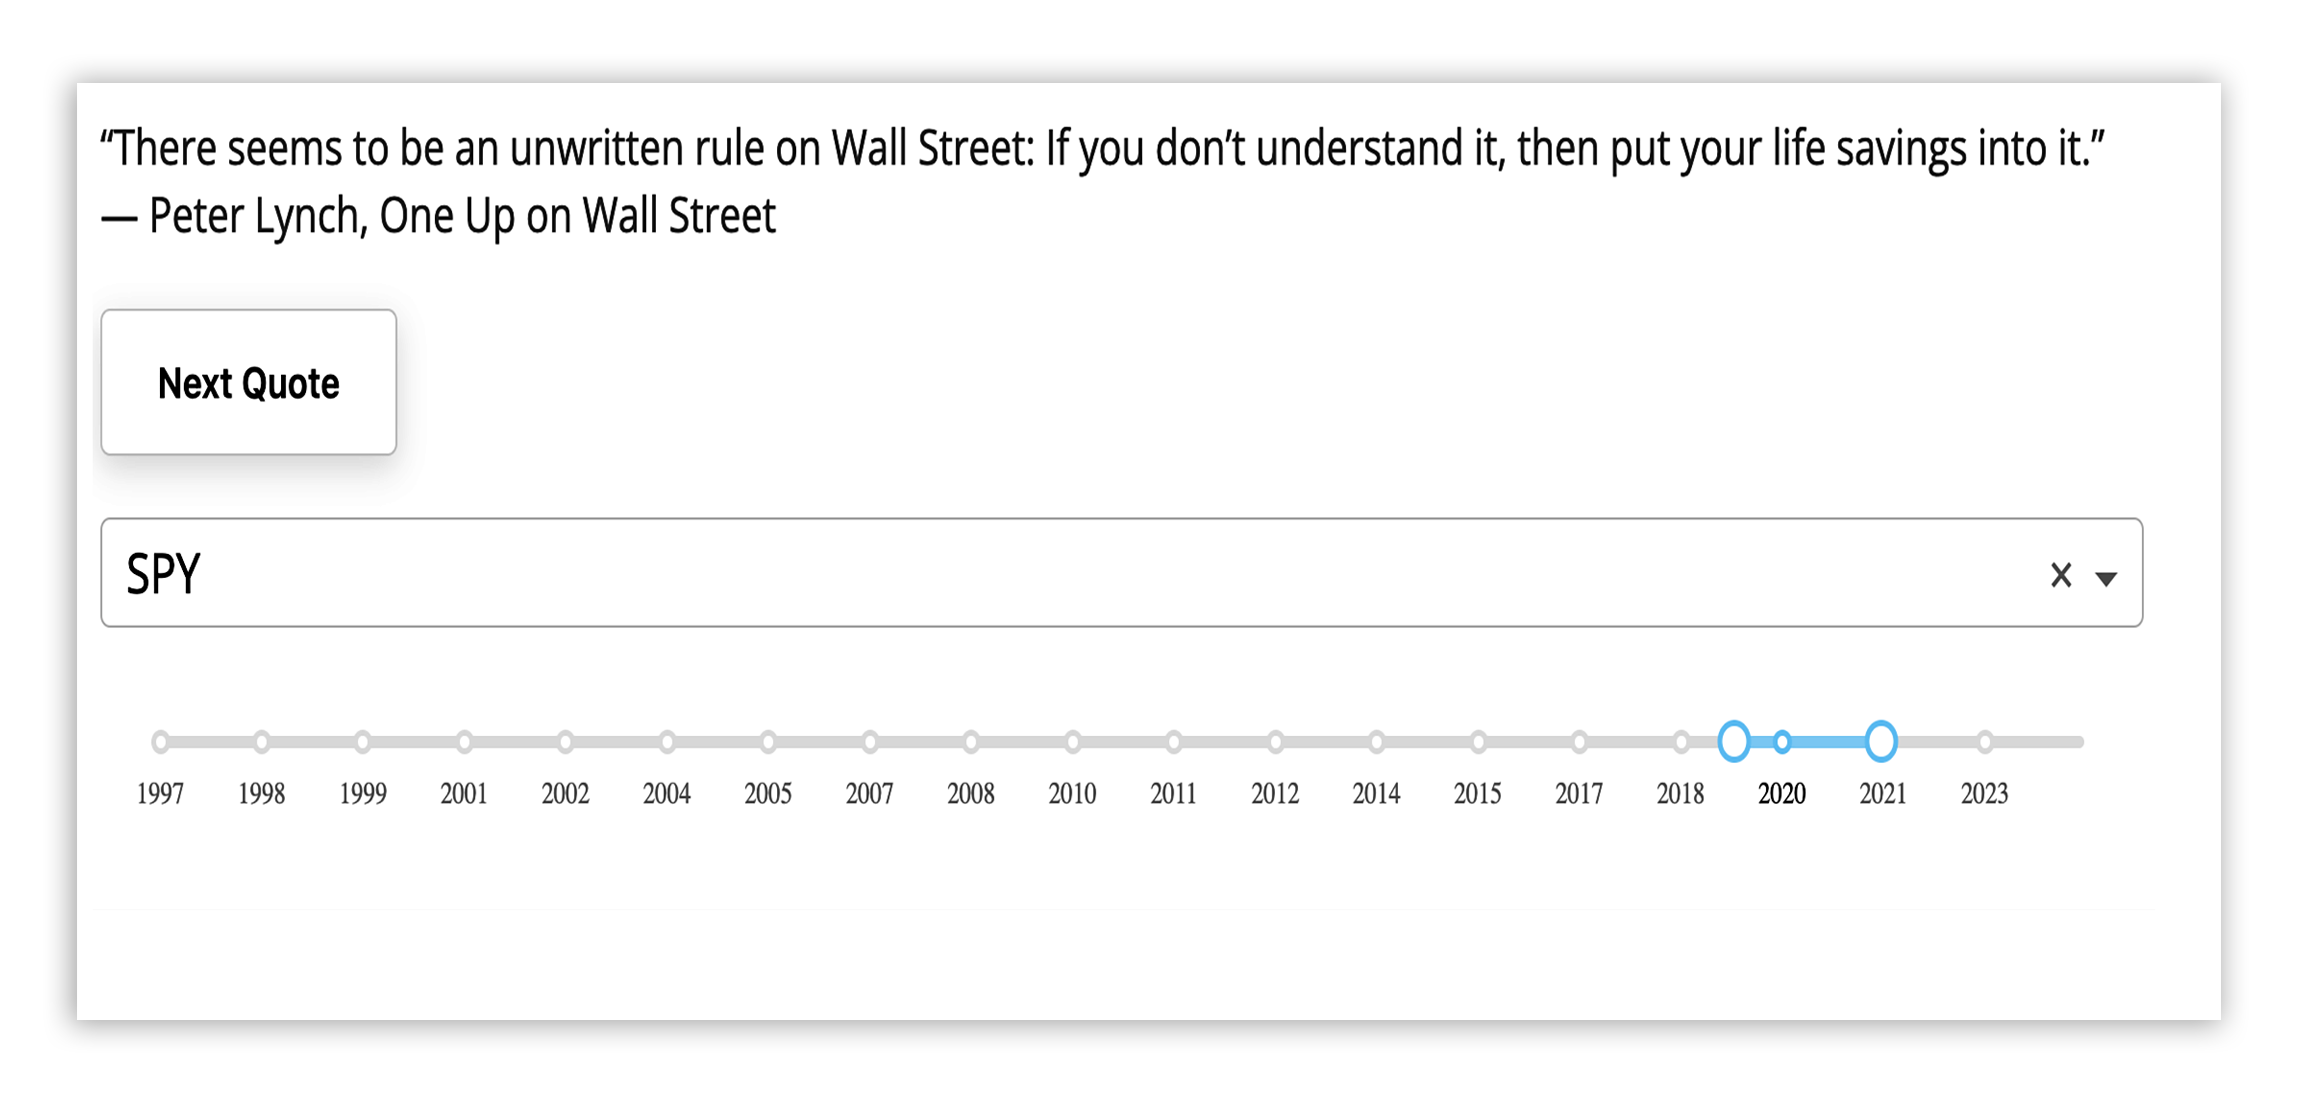
\includegraphics[width=\textwidth]{Figure_01.png}
    \caption{Reggie top of UI, showing quotation and date range slider.}
    \label{fig:fig1}
\end{figure*}

\begin{figure*}[h]
    \centering
    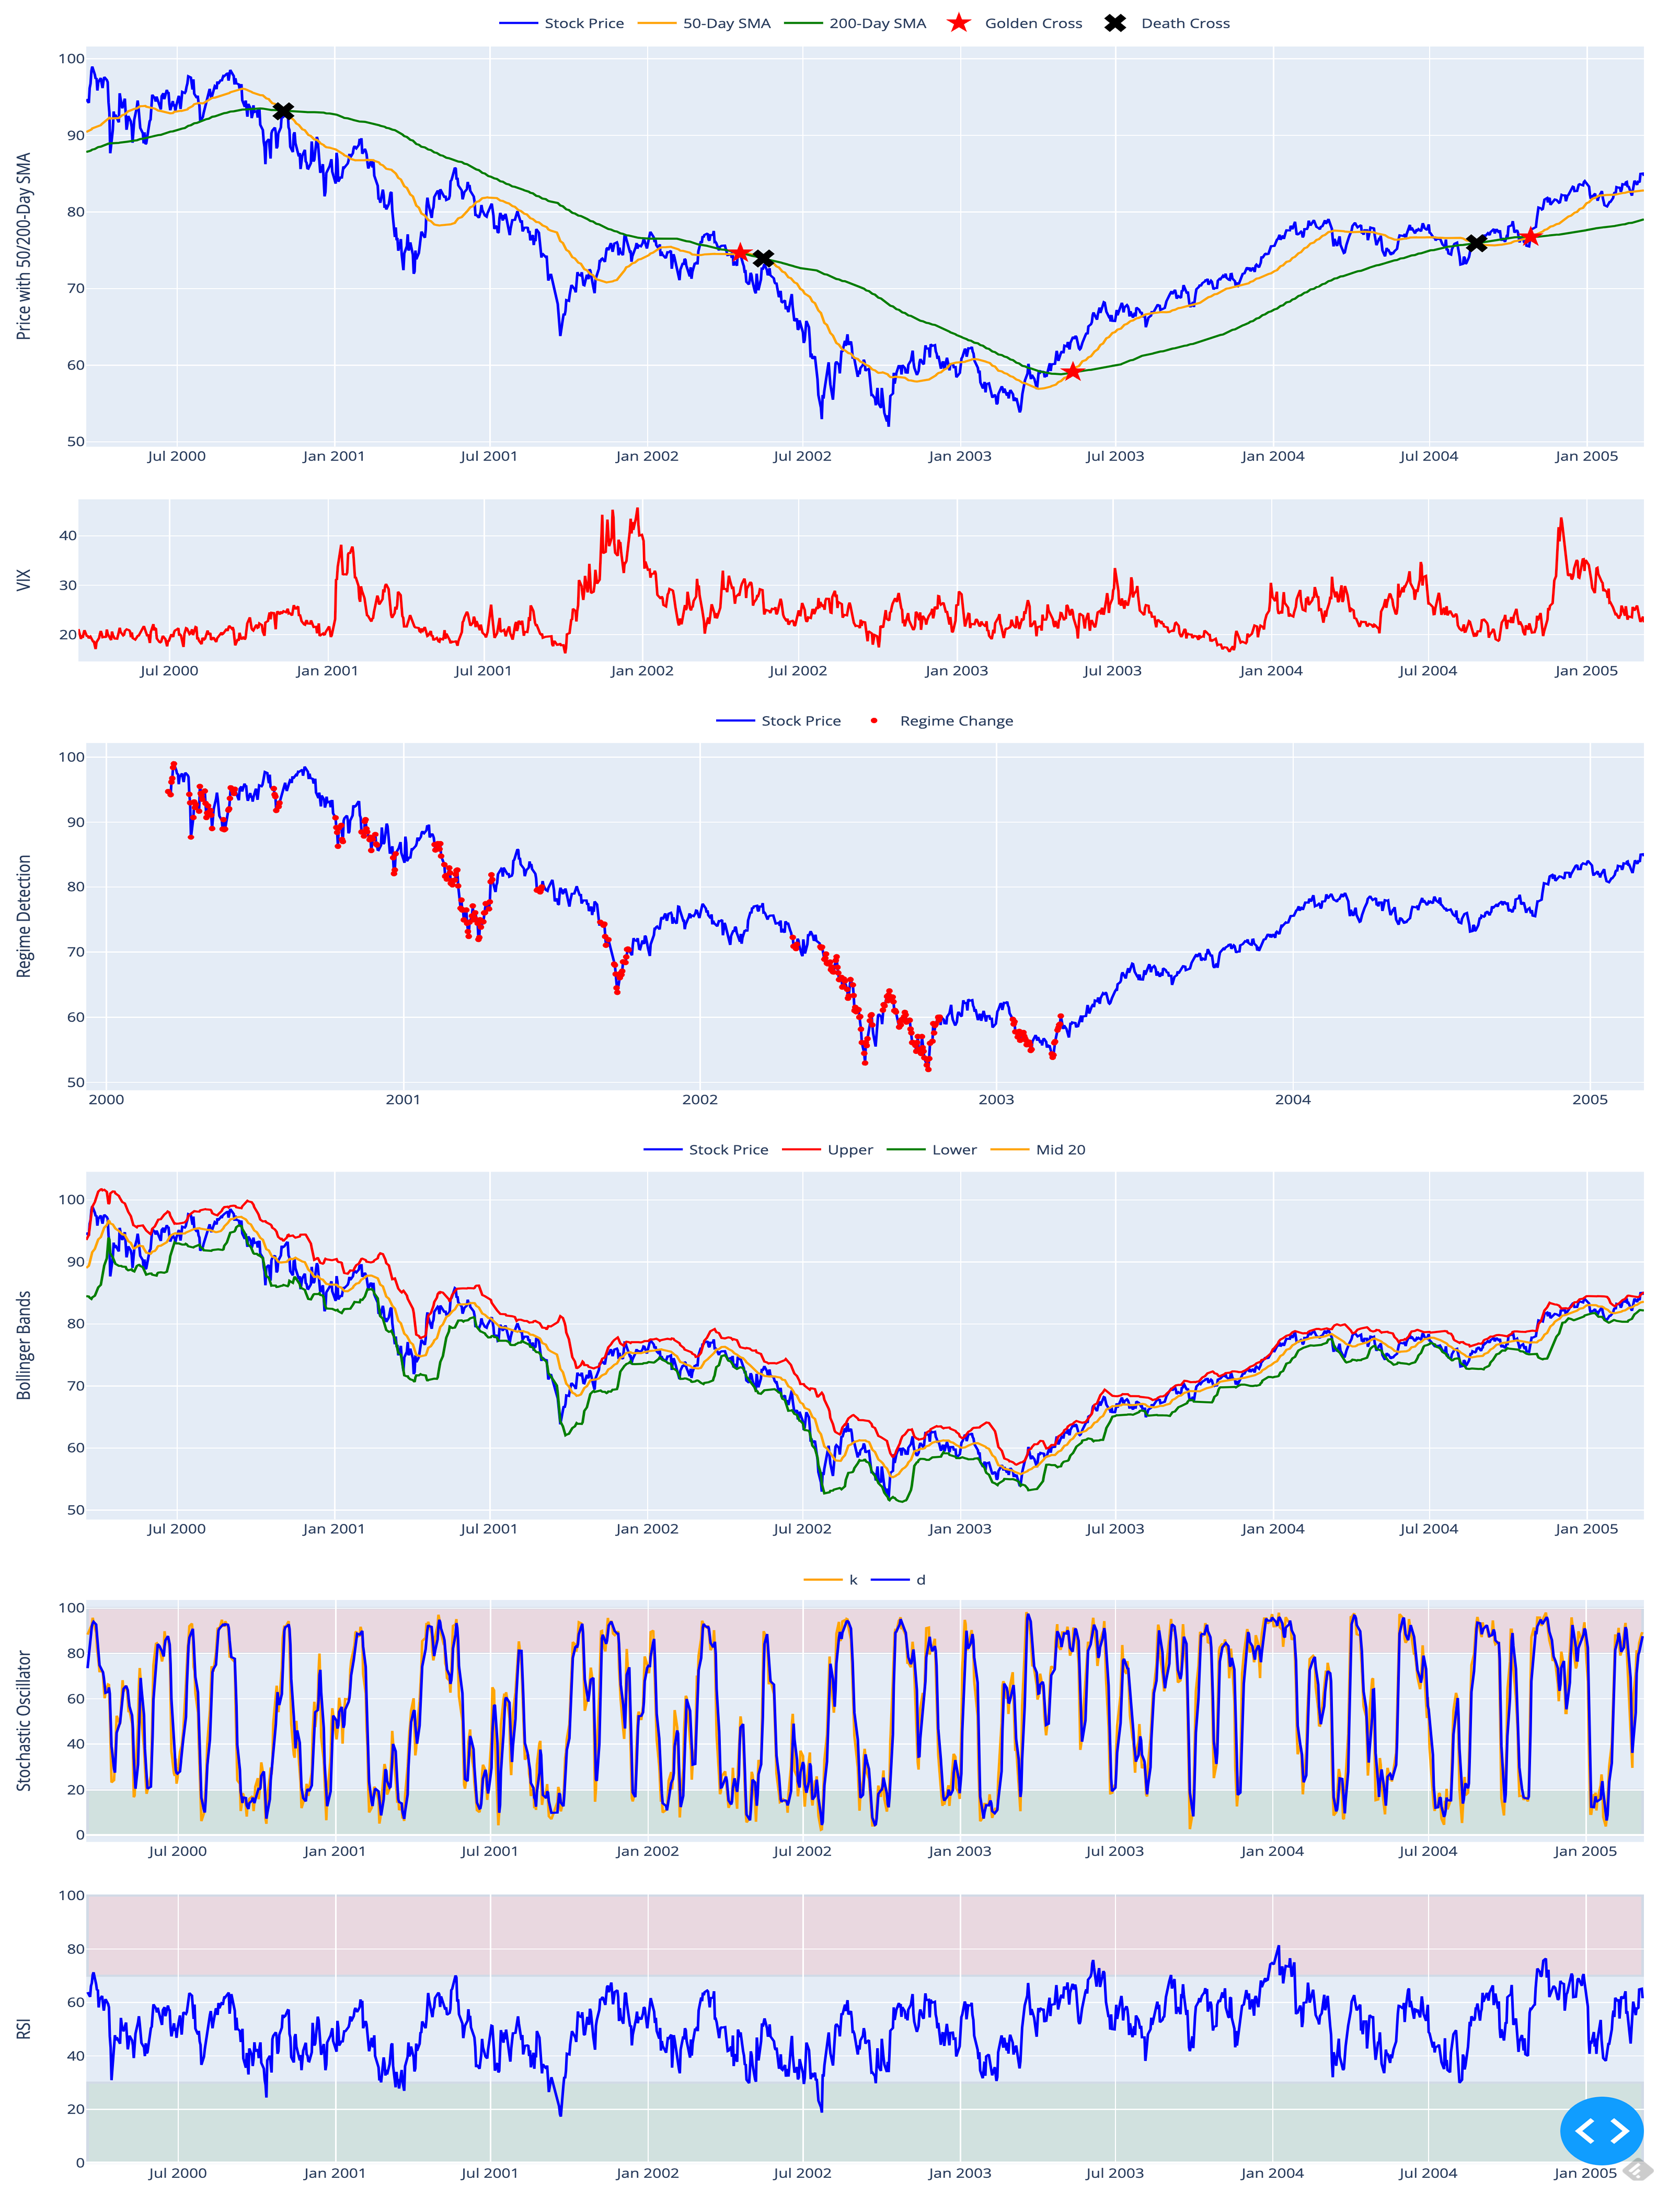
\includegraphics[width=\textwidth]{Figure_02.png}
    \caption{Dotcom Market Crash, March 2000 - March 2005.}
    \label{fig:fig2}
\end{figure*}

\begin{figure*}[h]
    \centering
    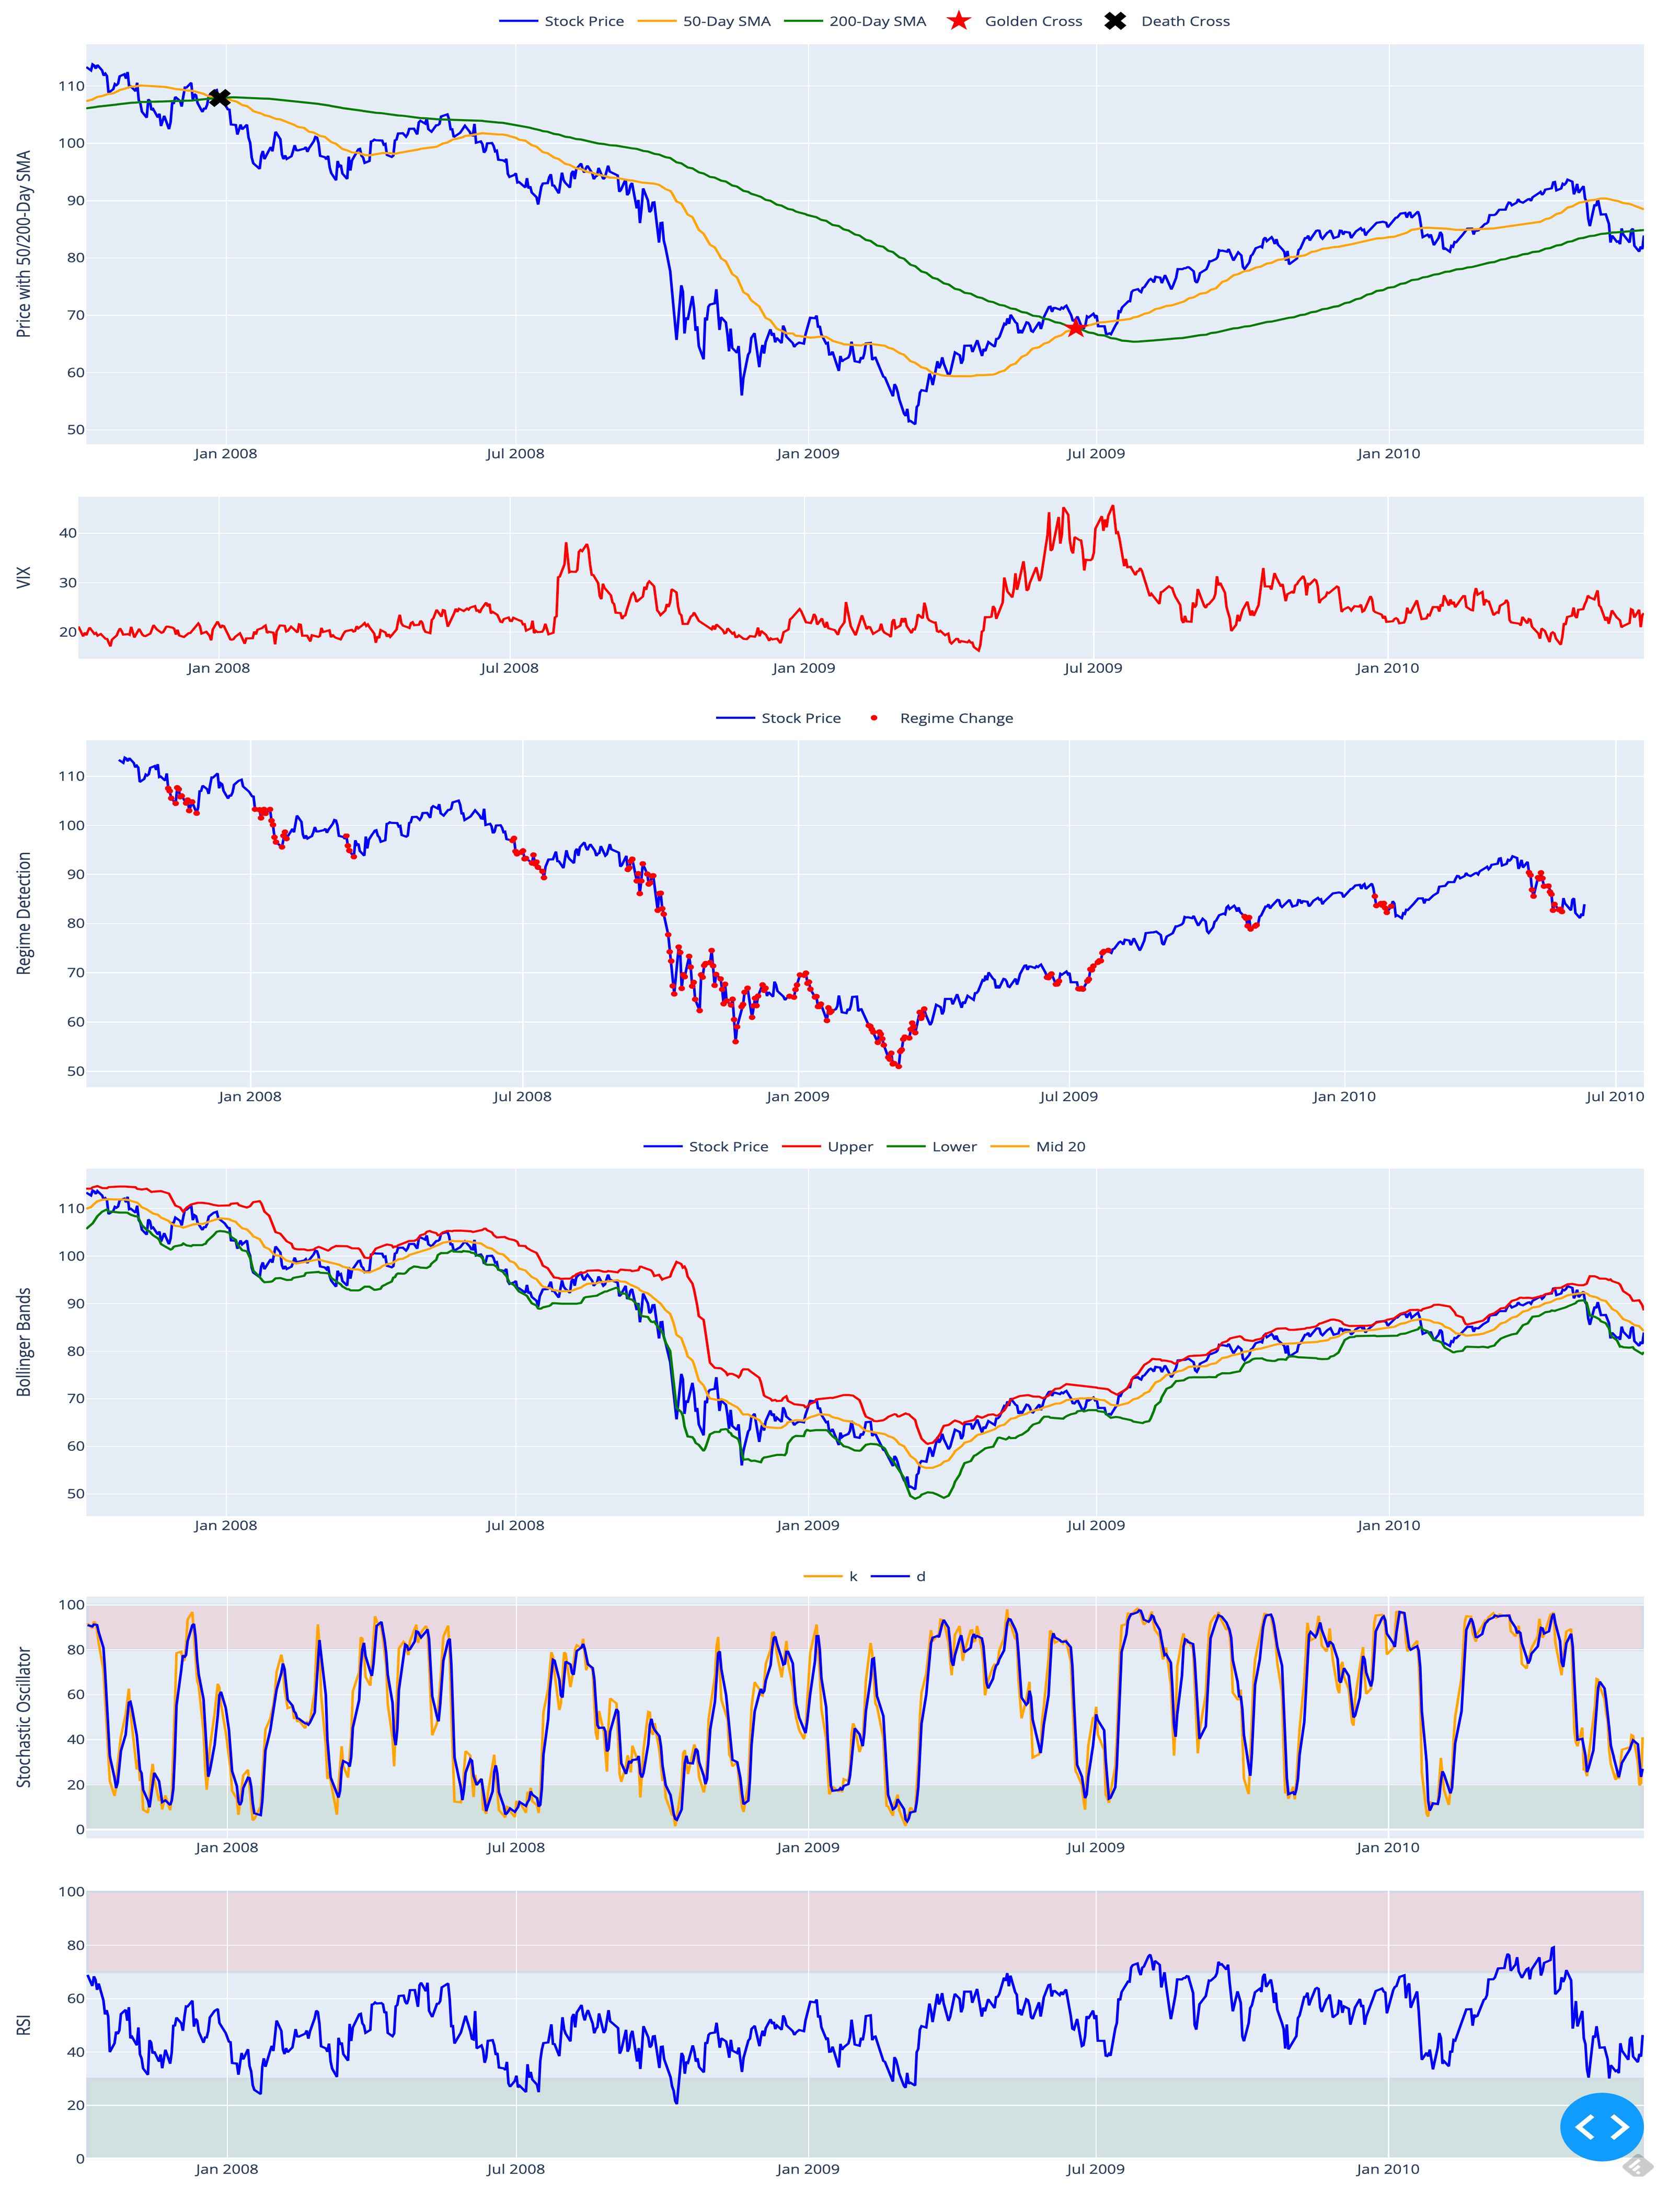
\includegraphics[width=\textwidth]{Figure_03.png}
    \caption{Global Financial Market Crash, October 2007 - June 2010}
    \label{fig:fig3}
\end{figure*}

\begin{figure*}[h]
    \centering
    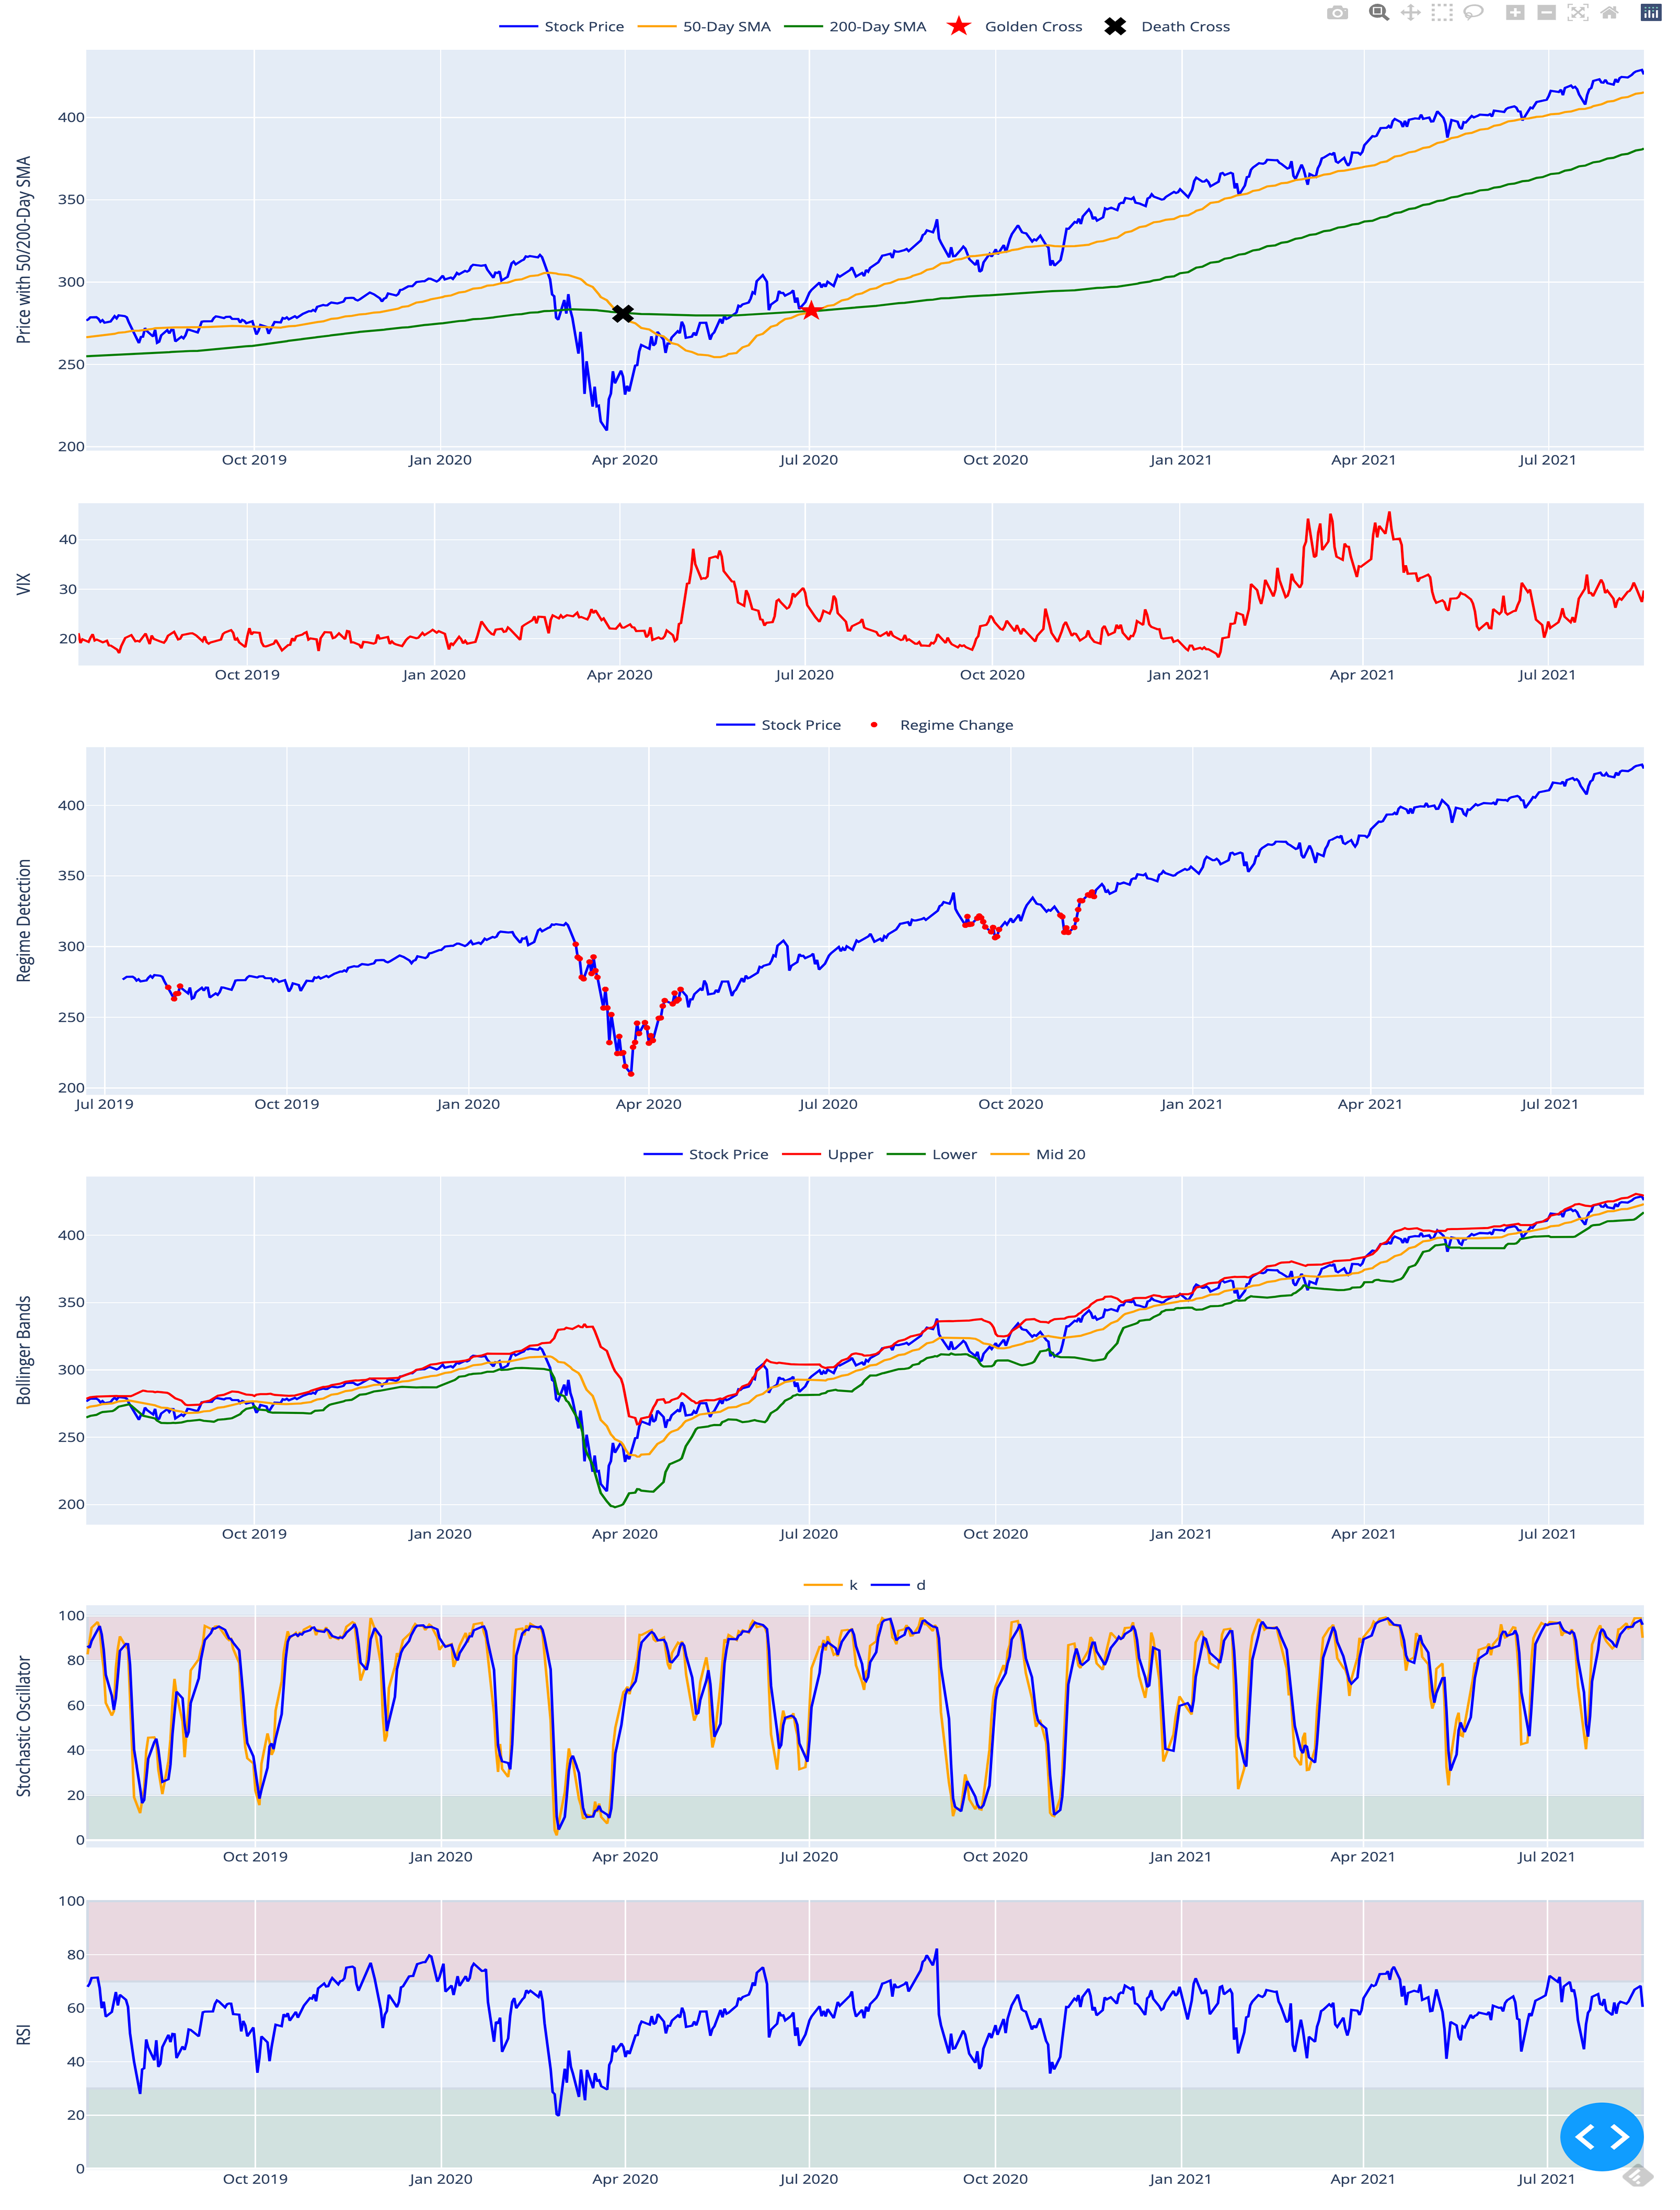
\includegraphics[width=\textwidth]{Figure_04.png}
    \caption{Covid Market Crash, July 2019 - August 2021}
    \label{fig:fig4}
\end{figure*}

\begin{figure*}[h]
    \centering
    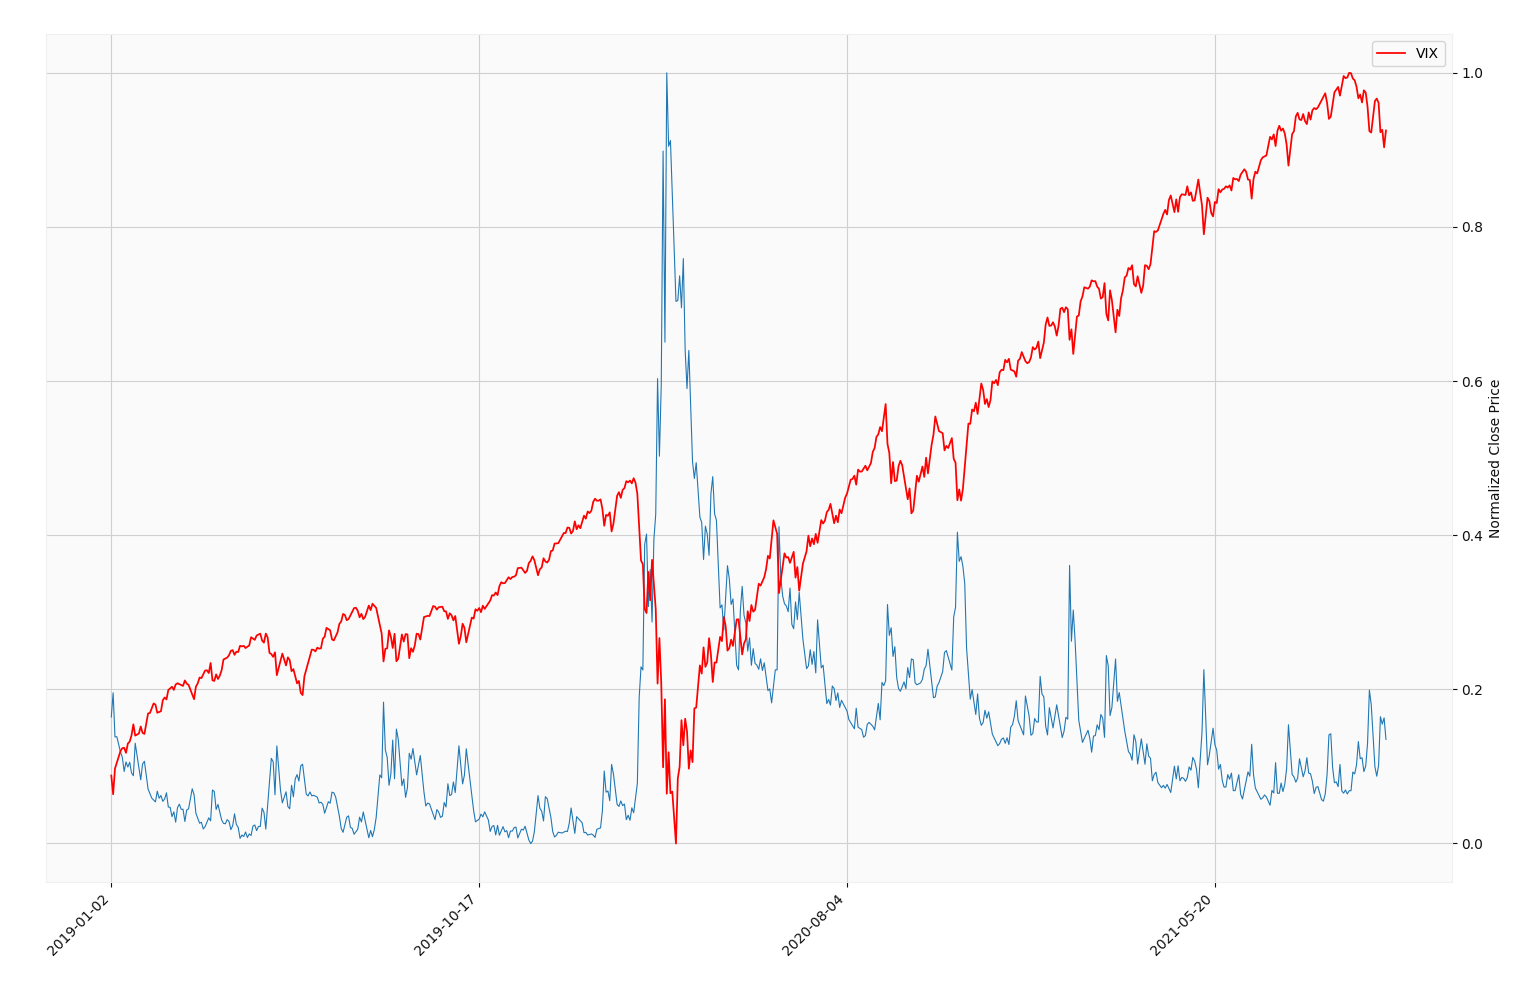
\includegraphics[width=\textwidth]{Figure_05.png}
    \caption{SPY and VIX Normalized for comparisson during the Pandemic Crash.}
    \label{fig:fig5}
\end{figure*}

\end{document}
